\documentclass[journal,letterpaper,twoside,twocolumn]{IEEEtran}

\usepackage{graphicx}
\usepackage[spanish]{babel}
\usepackage[utf8]{inputenc}
\usepackage[T1]{fontenc}
\usepackage{cite}

\graphicspath{{../images/}{./images/}}% pdflatex must be compiled from bin directory to mantain a clean repo 
\newcommand{\myreferences}{../../../doc/review/review/library}% SPECIFY THIS PATH!!!
\bibliographystyle{IEEEtran}% apsr, agsm, dcu, kluwer, nederlands

\title{Propuesta 1. Locomoción Humanoide:\\Contacto, Impacto y Dinámica Centroidal}
\author{Jaime Andrés~Castillo-León}
\markboth{Primera propuesta: Métodos de Simulación en Física}{Castillo-León: Locomoción Humanoide}

\begin{document}
\maketitle
\begin{abstract}
  En este documento se propone trabajar con dinámica multicuerpo, aplicada a una configuración humanoide utilizando el formalismo de los screws para describir la dínamica del centro de masa y el momento angular del sistema. La interacción con el entorno será llevada a cabo por el impacto y colisión de los pies, cuyo modelo será propuesto a partir de esferas. Además se propone una distribución de lo que sería el articulo final.
\end{abstract}
\begin{IEEEkeywords}
  Locomoción humanoide, Modelos de Impacto y Contacto, Dinamica Centroidal, Screws
\end{IEEEkeywords}

\section{Introducción}
\label{sec:intro}
\IEEEPARstart{P}{arte} de los problemas actuales de la simulación de la locomóción humanoide y sus aplicaciones a la biomecánica y las neurociencias, radíca en que los modelos de contacto y fricción actuales difieren bastante de la realidad\cite{Todorov2014}. Además la forma adecuada en que se describen y analizan la dinámica de la estructuras mecánicas, ha sido un reto para generar simulaciones en tiempo real\cite{Wensing2016}. Se ha probado diferentes formalismos: desde la mecánica clásica de las ecuaciónes de Newton-Euler, la mecánica analitica de Euler-Lagrange, los sistemas multipuertos de los Hamitonianos utilizando Bond Graphs o las ecuaciones de Kane partiendo del concepto de trabajo virtual. 

Generalmente cuando se utiliza el formalismo de Newton-Euler, para resolver la mecánica de cadenas cinemáticas tipo árbol, como las que se presentan en el cuerpo de los animales o en general de los seres vivos. Se debe plantear por cada cuerpo o eslabón que constituye a la cadena, seis ecuaciones de movimiento y luego se debe colocar restricciónes algebraicas para representar la física de las articulaciones, que finalmente representa la topología del mecanismo\cite{Taga1991}. Un motor físico, empleado para video juegos, ODE\cite{Smith2007}, soluciona las ecuaciones de movimiento, colision y friccion de esta forma, generando demasiadas ecuaciones. Se ha demostrado en varios artículos mediante benchmarks\cite{Sherman2011a,Erez2015} que este enfoque no es el adecuado para el análisis la locomoción de seres vivos\cite{Geijtenbeek2013,Wensing2015}.

Las ecuaciones de Euler-Lagrange producen un sistema de ecuaciones reducido, representado por variables generalizadas\cite{Spong2006}. A diferencia de Newton-Euler, el sistema a resolver es pequeño, lo cual para la síntesis de controladores es ventajoso a nivel computacional, no obstante este formalismo basado en el lagrangiano del sistema, no permite obtener de forma directa las fuerzas de interacción entre los cuerpos, las cuales son un requerimiento para el diseño mecánico del sistema. La topología de la cadena queda absorbida en el planteamiento del problema\cite{Featherstone2005}. Básicamente estos sistemas requiere de un motor algebraico diferencial para su solución, este motor se ejecuta como un preproceso y si la topología cambia se debe repetir el proceso\cite{Docquier2013}, situacion que no ocurre por Newton-Euler.

En el caso de los puertos Hamiltonianos, por ejemplo los Bond Graphs, representan un método gráfico para describir el flujo de energía del sistema, mediante dos variables: flujo y esfuerzo, además de la causalidad del sistema\cite{VanderSchaft2014}. La causalidad en este formalismo es utilizada para la implementación computacional automática de cómo deben ser planteadas y resueltas la ecuaciones de movimiento\cite{damic2015,Nageshrao2015b}. Una ventaja de los Bond Graphs es la aprarente sencilles con la que se puede acomplar diferentes medios físicos con el uso de los puertos, de allí que estos métodos se utilicen para problemas que involucran varios dominios físicos, como transferencia de calor, de masa, electromagnetismo y mecánica\cite{Nageshrao2015b}.

En este trabajo se propone utilizar un formalismo que puede moverse entre los cuatro anteriormente mencionados. Las ecuaciones de Lagrange son obtenidas a partir de algoritmos recursivos de Newton-Euler que a su vez son implementados utlizando el algebra de los Screws. Del sistema descrito en lagrangianos es posible obtener su representación en hamiltonianos y la construcción de las ecuaciones de Kane\cite{Liu2005a}. Los Screws permiten plantear las ecuaciones de movimiento de una forma más compacta y general, en donde se unen la translación y la rotación en una unica entidad matemática denomiada Screw\cite{Stramigioli2001}. La notación y construcción que se utilizará es la propuesta por Roy Feathrestone, en donde los Screws son definidos \emph{Vectores Espaciales} o \emph{6D-vectors}, con su respectiva algebra\cite{Featherstone2008,Featherstone2010b,Featherstone2010a}. Basicamente se definen dos tipos de Espacios Vectoriales: movimiento \emph{(Twist)} y fuerza \emph{(Wrenches)}\cite{Featherstone2006}.

Una vez son obtenidas las ecuaciones de movimiento por cualquier método, se debe resolver las ecuaciones diferenciales. Estas ecuaciones requieren que el solucionador tenga dos propiedades: (1) control de tamaño de paso adaptativo, para controlar el error y (2) resolver ecuaciones numéricamente rígidas (\emph{stiff}). Para esto las librerias Odeint\cite{Ahnert2011} de Boost desarrolladas bajo el paradigma de metaprogramación presente C++ serán utilizadas. Para la dinámica multicuerpo, la libreria RBDL\cite{Felis2016} en C++, implementa el trabajo de\cite{Featherstone2008}

\section{Simulación Multicuerpo}
\label{sec:simula}
El modelo del humanoide (ver Figura.\ref{fig:humModel}), consta de una cadena cinematica tipo árbol con base flotante y 34 grados de libertad. Los algoritmos de Featherstone para la solucion de la dínamica multicuerpo, en particular el algoritmo recursivo de \emph{cuerpos articulados}, con complejidad $\mathcal{O}(n)$ y $n$ los grados de libertad
\begin{figure}[!t]
  \centering
  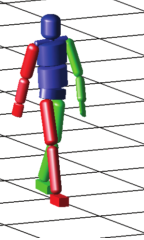
\includegraphics[scale=0.6]{Felis2016aHumanoidModel.png}
  \caption{Modelo humanoide \protect\cite{Felis2016a}.}
  \label{fig:humModel}
\end{figure}

\section{Modelos de Impacto y Contacto}
\label{sec:impYcon}
El modelo de fricción es una extensión del model de Hertz, que se ajusta mejora a datos experimentales\cite{Azad2010}. Incluye el modelo de Coulomb y efectos visco-elasticos sobre el cual se puede analizar la perdida de energía en el sistema. El pie se modela como se ilustra, ver Figura.\ref{fig:footModel}. 
\begin{figure}[!t]
  \centering
  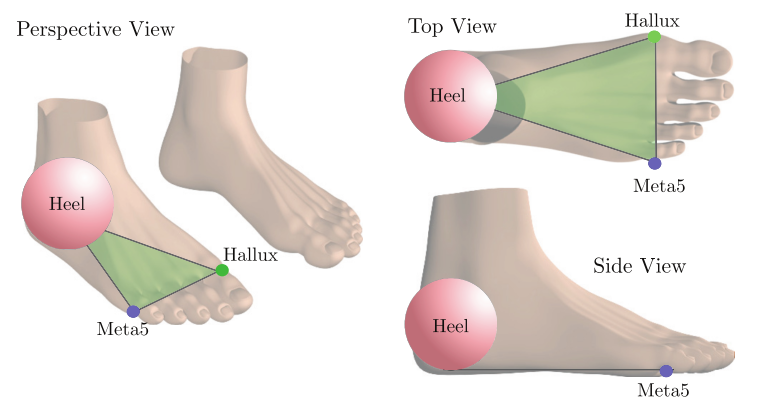
\includegraphics[scale=0.3]{Felis2016aFeetModel.png}
  \caption{Modelo del pie para el contacto y la colisión \protect\cite{Felis2016a}.}
  \label{fig:footModel}
\end{figure}

\section{Dinámica Centroidal}
\label{sec:dinCentr}
Se puede simplificar el analisis de las estructuras humanoides al simplificar las masa por su centro de masa e inercias equivalentes (ver Figura\ref{fig:footModel}), calculando el momento centronidal lineal y angular(ver Figura.\ref{fig:simpleModels}). 
\begin{figure}[!t]
  \centering
  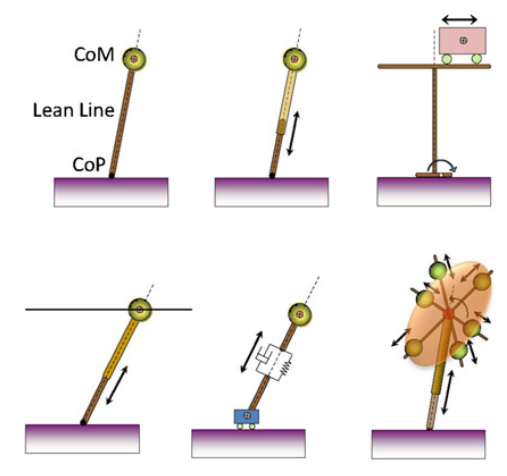
\includegraphics[scale=0.4]{Orin2013CentroidalDynamics.png}
  \caption{Modelos simplificados de humanoides \protect\cite{Orin2013}.}
  \label{fig:simpleModels}
\end{figure}
Existen varios espacios y transformaciones entre ellos, sobre los cuales es fácil sintetizar diferentes partes del control de un humanoide. En el espacio de la tarea se suele buscar las trayectorias adecuadas, mientras que las acciones de control estan en el espacio de configuración. El espacio de la dinamica centroidal es usado actualmente como referente para el diseño de las funciones objetivo que codifican los comportamientos del humanoide, que al final producen las trayectrorias deseadas por el robot\cite{Felis2016a,Wensing2016} (ver Figura.\ref{fig:diagTransf}).
\begin{figure}[!t]
  \centering
  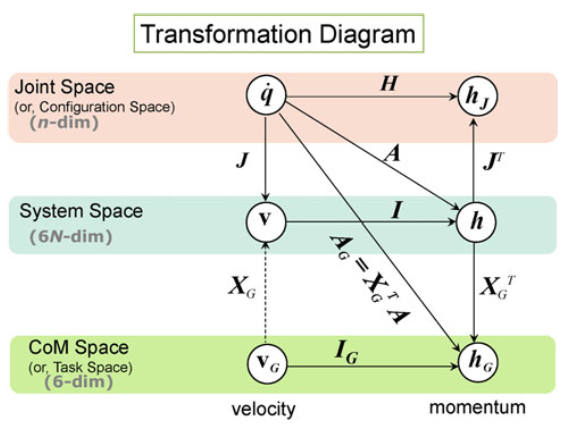
\includegraphics[scale=0.3]{Orin2013TransformationDiagram.png}
  \caption{Diagrama de transformaciones de espacio \protect\cite{Orin2013}.}
  \label{fig:diagTransf}
\end{figure}

\section{Generación de Trayectorias}
\label{sec:genTray}
Inicialmente se propone generación basada en ZMP\cite{Chen2011,Or2010}, pero para la segunda propuesta se propone aumentar el modelo del humanoide dotando con un sistema neuromuscular y utilizar métodos de control óptimo para la busqueda de las trayectorias, el cual es un trabajo de actualidad en este campo\cite{Peng2017}. 

\section{Discusión y Conclusiones}
\label{sec:conclu}

\section{Referencias}
\label{sec:refs}
\bibliography{\myreferences}

\end{document}
